\chapter{Introduction au calcul des cartes de reionisation}


Les cartes de redshift de reionization sont de outils important pour l'étude de la reionization dans son ensemble.
Ces cartes sont constituée en chaque point de l'espace, du redshift au quel chaque cellule et passer au dessus d'un certain niveau d'ionisation moyen.

Il est possible de définir deux façons d'allouer un redshift.
Il est possible de considérer la première, ou la dernière ionization.

Dans le cas de la première ionisation, la valeur ne devra être mise a jour qu'une seule fois au moment du passage du seuil.
Pour ce faire, toutes les cellules seront initialisées a une valeur impossible (prenons -1 pour l'exemple).
La mise a jour ne se fera donc qu'a la condition que la fraction d'ionisation soit superieure au seuil ET que la valeur actuelle du redshift d'ionisation soit -1.
Ainsi la valeur ne sera pas remise a jour a chaque pas de temps ou la cellule sera ionisée. 

Dans le cas de la dernière ionisation, la valeur du redshift sera mise a jour, tant que la fraction d'ionization de la cellule est inferieure au seuil.
Ainsi, si un cellule recombine, le valeur de son redshift associé sera de nouveau mise a jour, et la mise a jour stoppera a chaque passage au dessus du seuil.


Dans le cas d'une grille AMR, l'organisation de la grille est ammenée a évoluer.
La question du raffinement/deraffinement  se pose alors.
Si dans le cas du raffinement, l'injection directe du redshift de la cellule mère ne pose pas de problème particulier, les choses sont différentes lors du déraffinement.
En effet, dans EMMA, quand une cellule est deraffinée la valeur moyenne des 8 cellules filles est injectée dans la cellule mère.
Le problème est que les redshift ne doivent pas être moyennés.
La simulation, et les processus physiques qui y ont lieu, sont calculé par rapport au temps.
Nous avons vu dans la partie (TODO ref) qu'il existe un lien non trivial entre le redshift et temps (l'age de l'Univers).
Pour répondre a ce problème, j'ai fait le choix de travailler non pas avec le redshift mais avec l'age de l'Univers au moment de l'ionisation de la cellule.
Les cartes de temps seront converties en cartes de redshift en post traitement en utilisant les meme paramètres cosmologique que ceux du run.



\begin{figure}[htpb]
        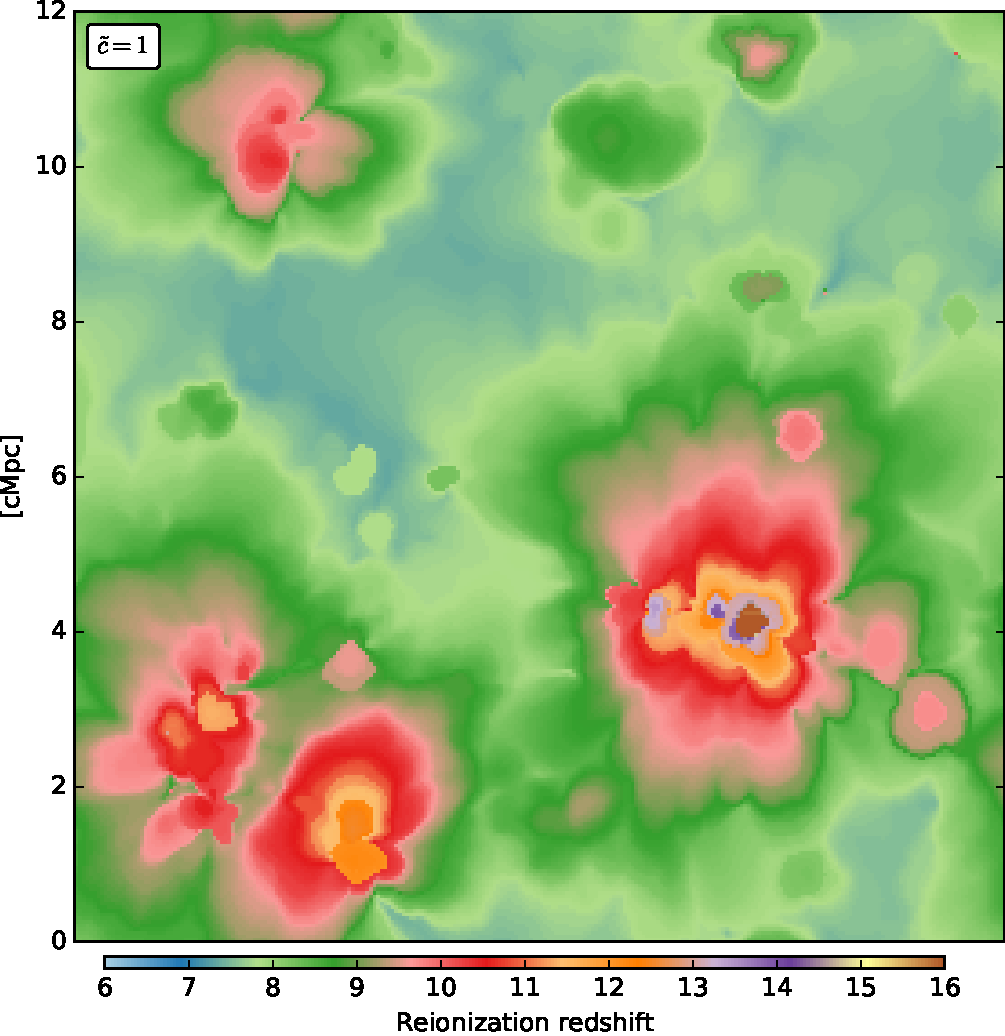
\includegraphics[width=.95\linewidth]{img/04_mapreio/map_z_c1.pdf} 
        \caption{ }
 		\label{}
\end{figure}


\begin{figure}[htpb]
        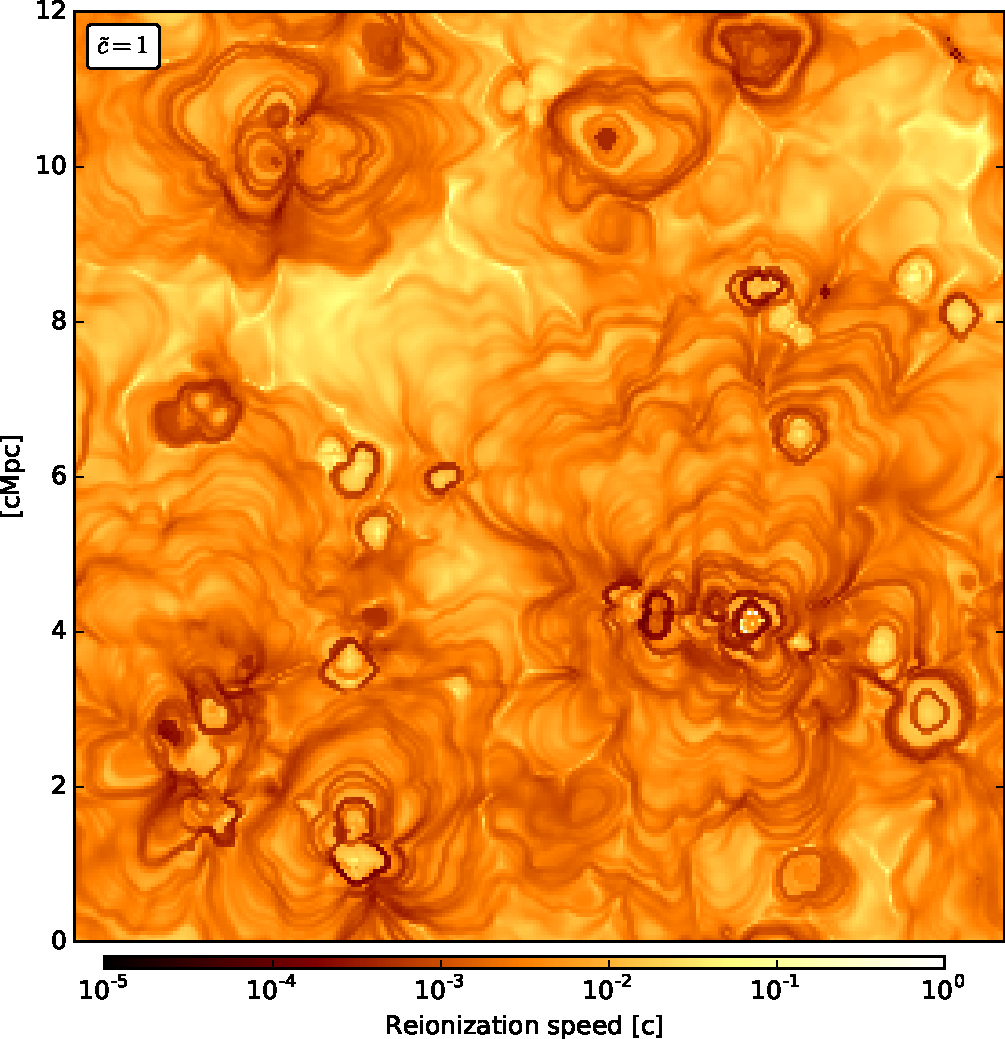
\includegraphics[width=.95\linewidth]{img/04_mapreio/map_v_c1.pdf} 
        \caption{ }
 		\label{}
\end{figure}